\begin{figure*}[!h]
\begin{subfigure}{0.27\linewidth}
\centering
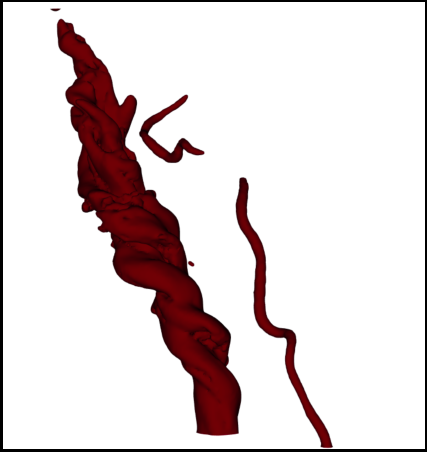
\includegraphics[width=0.9\linewidth]{Images/Tornado/zls.pdf}
\vspace{-2mm}
\caption{$ZLS_{T}$}
\label{fig:tornado_zls}
\end{subfigure}
\begin{subfigure}{0.27\linewidth}
\centering
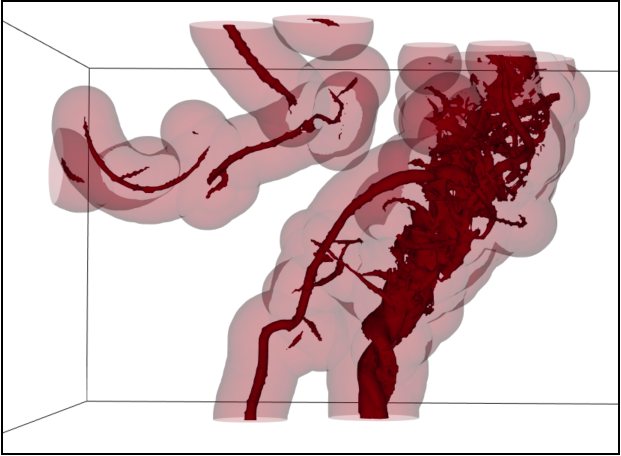
\includegraphics[width=0.9\linewidth]{Images/Tornado/fls_05.pdf}
\vspace{-2mm}
\caption{$ZLS_{T}$ + $FLS_{T,0.5}$}
\label{fig:tornado_fls}
\end{subfigure}
\begin{subfigure}{0.27\linewidth}
\centering
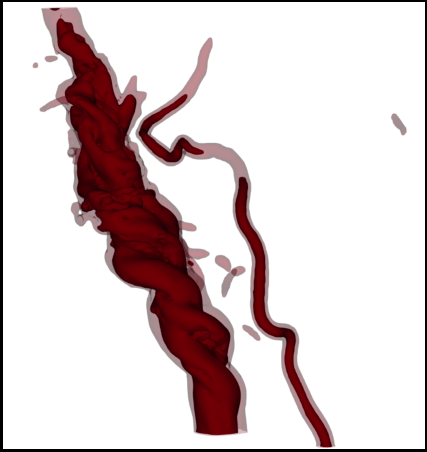
\includegraphics[width=0.9\linewidth]{Images/Tornado/fcls_68.pdf}
\vspace{-2mm}
\caption{$ZLS_{T}$ + $FCLS_{T,68\%}$}
\label{fig:tornado_fcls}
\end{subfigure}
\hfill
\begin{subfigure}{0.17\linewidth}
\centering
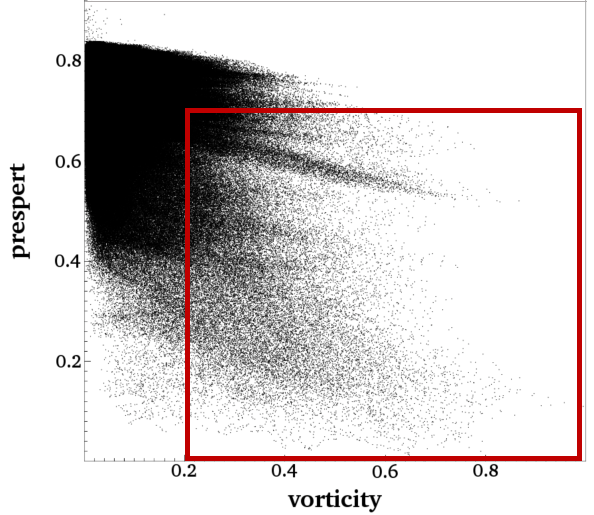
\includegraphics[width=\linewidth]{Images/Tornado/scatterplot.pdf}
\vspace{-4mm}
\caption{Attribute space 2D scatterplot and trait (rectangular selection).} 
\label{fig:tornado_scatterplot}
\end{subfigure}
\vspace{-2mm}
\caption{Visualization of EF-5 tornado vortices using vorticity magnitude and pressure pertubation attributes.}
%\vspace{-1mm}
\label{fig:tornado}
\end{figure*}
